\documentclass[12pt, a4paper]{article}

\usepackage[medium]{titlesec}
\usepackage{graphicx}
\usepackage{caption}
\usepackage{amsmath}
\usepackage{amsthm}
\usepackage[legalpaper, portrait, margin=1.2in]{geometry}
\usepackage{wrapfig}
\usepackage{varwidth}
\usepackage{listings}
\usepackage{amssymb}
\usepackage{enumitem}
\usepackage{bm}
\usepackage{enumitem}

\allowdisplaybreaks  % will allow page break in align environment

\begin{document}
	
	\setlength{\parindent}{0pt}
	\captionsetup{justification=centering}
	\lstset{
		showstringspaces=false
	}
	
	
	\begin{titlepage}
		\LARGE
		\textbf{7.5}
		\begin{center}
			\vspace*{7cm}
			
			\LARGE
			\textbf{Mathematical Methods}
			\\
			\vspace{1cm}
			\textbf{Pad\'e Approximants}
			
			\vspace{0.5cm}
		\end{center}
	\end{titlepage}

\section{Introduction}	
	
\subsubsection*{Programming Task: Writing Programs A and B}

The programs written for this task can be found on pages \pageref{Program_A} and \
\pageref{Program_B}. From the numpy package in Python, I use the \texttt{lstsq} function \
as an equivalent of \texttt{mldivide} from Matlab. I first tested Program A for basic \
functions such as f(x) = 0 with different values of L and M. Then I carried out testing \
with more complex functions such as f(x) = sin(x) and confirming the $O(x^{L+M+1})$ \
accuracy via polynomial division of the results.


\subsubsection*{Question 1}

Using the binomial expansion, we obtain,
\begin{flalign*}
	f_{1}(x) = 1 + \frac{x}{2} - \frac{x^{2}}{8} + \frac{x^{3}}{16} &&
\end{flalign*}
with the following formula for the coefficients,
\begin{flalign*}
	c_{0} = 1, \quad c_{1} = \frac{1}{2}, \quad c_{k} = \frac{ (-1)^{k-1}(2k-3)! }{ 2^{2k-2}k!(k-2)! } \text{ for } \ 
	k \geq 1. &&
\end{flalign*}

The radius of convergence can be found via the ratio test.
\begin{flalign*}
	\text{Radius} & = \lim_{k \to \infty} \left| \frac{ c_{k} }{ c_{k+1} } \right| &&\\
	& = \lim_{k \to \infty}\left| \frac{ (2k-1)(2k-2) }{ 4(k+1)(k-1) } \right| &&\\
	& = 1
\end{flalign*}
This means that the Pad\'e approximant will only be useful within the disk of radius 1 \ 
centred at 0 in the complex plane. Also, the further from 0 you go, the more terms of \ 
the power series are required for a precise result. Therefore, approximants with a \ 
lower value of L+M+1 become much less useful in these cases.
\\

Taking $x = 1$ in the power series, we obtain $\sum_{k = 0}^{\infty}c_{k}$. Since this converges, the \
sequence of partial sums $\sum_{k = 0}^{N}c_{k}$ converges. This convergence is illustrated in figure\ 
\ref{q1_fig1}

\vspace{0.3cm}
\begin{minipage}{\textwidth}
	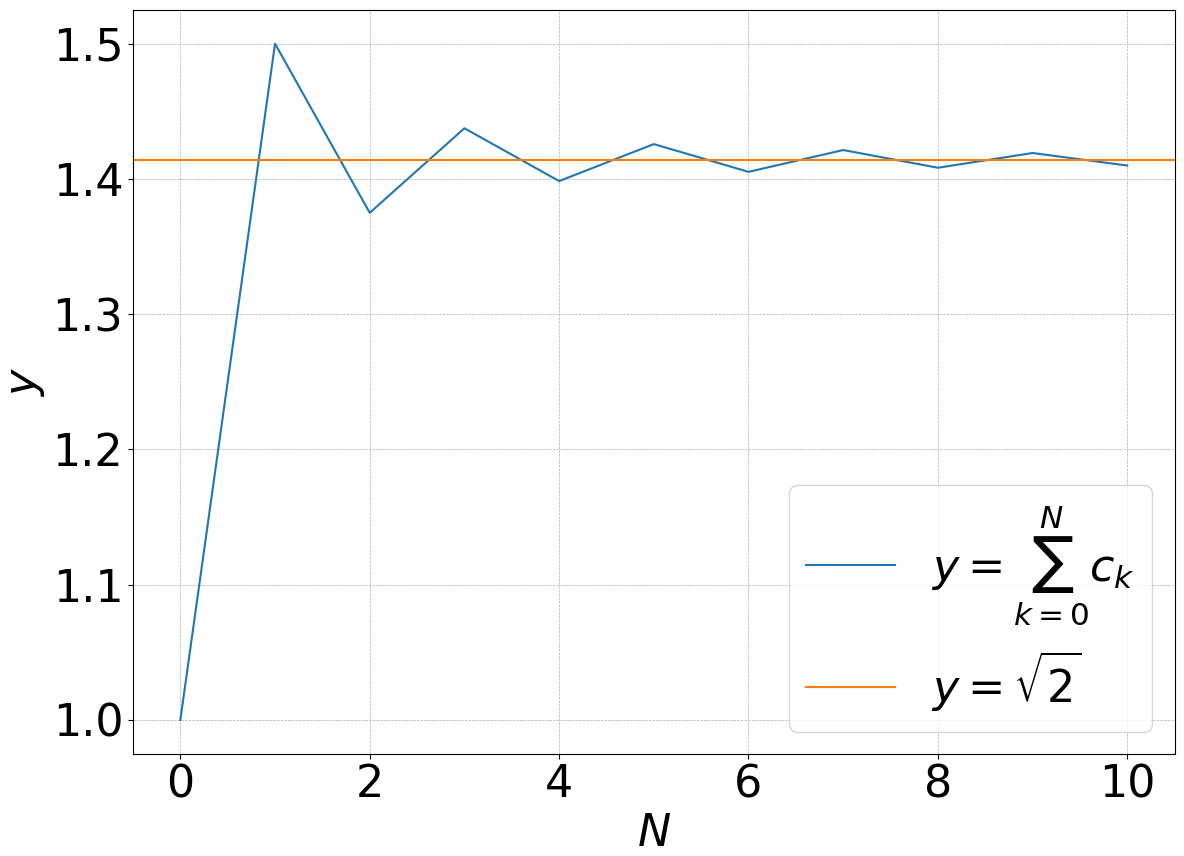
\includegraphics[width=\linewidth]{q1_fig1}
	\captionof{figure}{Line graph of partial sums}
	\label{q1_fig1}
\end{minipage}
\vspace{0.1cm}

We notice that the partial sums oscillate above and below $\sqrt{2}$, with the error growing smaller\
as $k$ increases. \\

$c_{k} = (1 - \frac{3}{2k})c_{k-1}$. 


\subsubsection*{Question 2}

	

\pagebreak
\textbf{Program\textunderscore A.py for Programming Task}\centering\label{Program_A}
\lstinputlisting[language=Python]{C:/Users/angus/OneDrive/Documents/CATAM 7.5/Program_A.py}
\vspace{2cm}

\pagebreak
\textbf{Program\textunderscore B.py for Programming Task}\centering\label{Program_B}
\lstinputlisting[language=Python]{C:/Users/angus/OneDrive/Documents/CATAM 7.5/Program_B.py}
\vspace{2cm}


\end{document}